\documentclass[tikz,border=20pt]{standalone}
\usetikzlibrary{calc,arrows.meta,positioning,shapes.geometric,fit}
\usepackage{amsmath,amssymb}

\definecolor{attenorange}{HTML}{FED7AA}
\definecolor{attentext}{HTML}{9A3412}
\definecolor{ffnblue}{HTML}{BAE6FD}
\definecolor{ffntext}{HTML}{075985}
\definecolor{normyellow}{HTML}{FEF08A}
\definecolor{normtext}{HTML}{854D0E}
\definecolor{embedpink}{HTML}{FBCFE8}
\definecolor{embedtext}{HTML}{831843}
\definecolor{lineargreen}{HTML}{BBF7D0}
\definecolor{lineartext}{HTML}{15803D}

\begin{document}
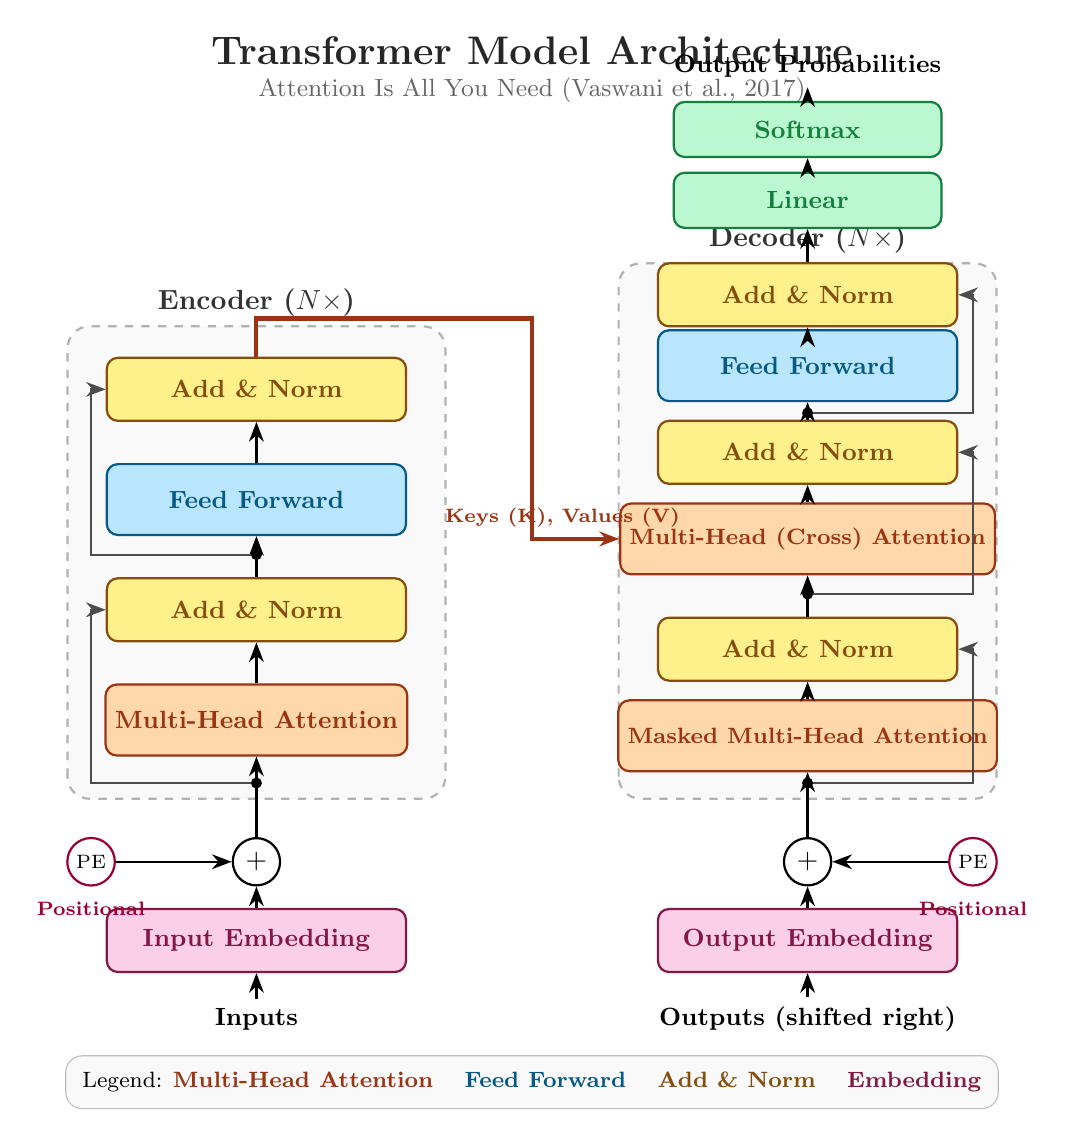
\begin{tikzpicture}[
  x=1cm, y=1cm, >=Stealth,
  mhablock/.style={rectangle, draw=attentext, fill=attenorange, thick, rounded corners=4pt, text centered, minimum width=3.8cm, minimum height=0.9cm, font=\bfseries\small, text=attentext},
  ffnblock/.style={rectangle, draw=ffntext, fill=ffnblue, thick, rounded corners=4pt, text centered, minimum width=3.8cm, minimum height=0.9cm, font=\bfseries\small, text=ffntext},
  normblock/.style={rectangle, draw=normtext, fill=normyellow, thick, rounded corners=4pt, text centered, minimum width=3.8cm, minimum height=0.8cm, font=\bfseries\small, text=normtext},
  embedblock/.style={rectangle, draw=embedtext, fill=embedpink, thick, rounded corners=4pt, text centered, minimum width=3.8cm, minimum height=0.8cm, font=\bfseries\small, text=embedtext},
  line/.style={draw, thick, -{Stealth[length=2.5mm]}}
]

  % Title
  \node[font=\bfseries\Large, text=black!85] at (5.0, 7.5) {Transformer Model Architecture};
  \node[font=\small, text=gray!80!black] at (5.0, 7.0) {Attention Is All You Need (Vaswani et al., 2017)};

  % ==================== ENCODER STACK (Left: X = 1.5) ====================
  % Inputs
  \node[font=\bfseries\small] (enc_in) at (1.5, -4.8) {Inputs};
  \node[embedblock] (enc_emb) at (1.5, -3.8) {Input Embedding};
  \node[circle, draw=black, thick, fill=white, inner sep=0pt, minimum size=6mm] (enc_plus) at (1.5, -2.8) {$+$};

  % Positional encoding
  \node[circle, draw=purple!80!black, thick, fill=white, inner sep=2pt, font=\scriptsize] (enc_pe) at (-0.6, -2.8) {PE};
  \node[font=\scriptsize\bfseries, text=purple!80!black, below=2pt of enc_pe] {Positional};

  \draw[line] (enc_in) -- (enc_emb);
  \draw[line] (enc_emb) -- (enc_plus);
  \draw[line] (enc_pe) -- (enc_plus);

  % Outer Encoder Box
  \draw[gray!60, thick, dashed, fill=gray!5, rounded corners=8pt] (-0.9, -2.0) rectangle (3.9, 4.0);
  \node[font=\bfseries\normalsize, text=black!80] at (1.5, 4.3) {Encoder ($N\times$)};

  % Encoder Layers
  \node[mhablock] (enc_mha) at (1.5, -1.0) {Multi-Head Attention};
  \node[normblock] (enc_norm1) at (1.5, 0.4) {Add \& Norm};
  \node[ffnblock] (enc_ffn) at (1.5, 1.8) {Feed Forward};
  \node[normblock] (enc_norm2) at (1.5, 3.2) {Add \& Norm};

  \draw[line] (enc_plus) -- (enc_mha);
  \draw[line] (enc_mha) -- (enc_norm1);
  \draw[line] (enc_norm1) -- (enc_ffn);
  \draw[line] (enc_ffn) -- (enc_norm2);

  % Residual 1
  \draw[line, gray!60!black] (1.5, -1.8) -| (-0.6, 0.4) -- (enc_norm1.west);
  \fill[black] (1.5, -1.8) circle (2pt);

  % Residual 2
  \draw[line, gray!60!black] (1.5, 1.1) -| (-0.6, 3.2) -- (enc_norm2.west);
  \fill[black] (1.5, 1.1) circle (2pt);


  % ==================== DECODER STACK (Right: X = 8.5) ====================
  % Outputs
  \node[font=\bfseries\small] (dec_in) at (8.5, -4.8) {Outputs (shifted right)};
  \node[embedblock] (dec_emb) at (8.5, -3.8) {Output Embedding};
  \node[circle, draw=black, thick, fill=white, inner sep=0pt, minimum size=6mm] (dec_plus) at (8.5, -2.8) {$+$};

  % Positional encoding
  \node[circle, draw=purple!80!black, thick, fill=white, inner sep=2pt, font=\scriptsize] (dec_pe) at (10.6, -2.8) {PE};
  \node[font=\scriptsize\bfseries, text=purple!80!black, below=2pt of dec_pe] {Positional};

  \draw[line] (dec_in) -- (dec_emb);
  \draw[line] (dec_emb) -- (dec_plus);
  \draw[line] (dec_pe) -- (dec_plus);

  % Outer Decoder Box
  \draw[gray!60, thick, dashed, fill=gray!5, rounded corners=8pt] (6.1, -2.0) rectangle (10.9, 4.8);
  \node[font=\bfseries\normalsize, text=black!80] at (8.5, 5.1) {Decoder ($N\times$)};

  % Decoder Layers
  \node[mhablock] (dec_mmha) at (8.5, -1.2) {\footnotesize Masked Multi-Head Attention};
  \node[normblock] (dec_norm1) at (8.5, -0.1) {Add \& Norm};
  \node[mhablock] (dec_cross) at (8.5, 1.3) {\footnotesize Multi-Head (Cross) Attention};
  \node[normblock] (dec_norm2) at (8.5, 2.4) {Add \& Norm};
  \node[ffnblock] (dec_ffn) at (8.5, 3.5) {Feed Forward};
  \node[normblock] (dec_norm3) at (8.5, 4.4) {Add \& Norm};

  \draw[line] (dec_plus) -- (dec_mmha);
  \draw[line] (dec_mmha) -- (dec_norm1);
  \draw[line] (dec_norm1) -- (dec_cross);
  \draw[line] (dec_cross) -- (dec_norm2);
  \draw[line] (dec_norm2) -- (dec_ffn);
  \draw[line] (dec_ffn) -- (dec_norm3);

  % Decoder Residual 1
  \draw[line, gray!60!black] (8.5, -1.8) -| (10.6, -0.1) -- (dec_norm1.east);
  \fill[black] (8.5, -1.8) circle (2pt);

  % Decoder Residual 2
  \draw[line, gray!60!black] (8.5, 0.6) -| (10.6, 2.4) -- (dec_norm2.east);
  \fill[black] (8.5, 0.6) circle (2pt);

  % Decoder Residual 3
  \draw[line, gray!60!black] (8.5, 2.9) -| (10.6, 4.4) -- (dec_norm3.east);
  \fill[black] (8.5, 2.9) circle (2pt);

  % CROSS ATTENTION FEED: Encoder Output -> Decoder Cross-Attention
  \draw[line, attentext, line width=1.5pt] (enc_norm2.north) -- (1.5, 4.1) -- (5.0, 4.1) -- (5.0, 1.3) -- (dec_cross.west)
    node[pos=0.35, above, font=\scriptsize\bfseries] {Keys (K), Values (V)};

  % OUTPUT STAGE (Linear, Softmax, Probabilities)
  \node[rectangle, draw=lineartext, fill=lineargreen, thick, rounded corners=4pt, font=\bfseries\small, text=lineartext, minimum width=3.4cm, minimum height=0.7cm] (linear) at (8.5, 5.6) {Linear};
  \node[rectangle, draw=lineartext, fill=lineargreen, thick, rounded corners=4pt, font=\bfseries\small, text=lineartext, minimum width=3.4cm, minimum height=0.7cm] (softmax) at (8.5, 6.5) {Softmax};
  \node[font=\bfseries\small] (prob) at (8.5, 7.3) {Output Probabilities};

  \draw[line] (dec_norm3) -- (linear);
  \draw[line] (linear) -- (softmax);
  \draw[line] (softmax) -- (prob);

  % Legend
  \node[draw=gray!50, fill=gray!5, rounded corners=6pt, font=\footnotesize, inner sep=6pt] at (5.0, -5.6) {
    Legend: \textcolor{attentext}{\textbf{Multi-Head Attention}} \quad \textcolor{ffntext}{\textbf{Feed Forward}} \quad \textcolor{normtext}{\textbf{Add \& Norm}} \quad \textcolor{embedtext}{\textbf{Embedding}}
  };

\end{tikzpicture}
\end{document}
